\documentclass[]{article}

% Imported Packages
%------------------------------------------------------------------------------
\usepackage{amssymb}
\usepackage{amstext}
\usepackage{amsthm}
\usepackage{amsmath}
\usepackage{enumerate}
\usepackage{fancyhdr}
\usepackage[margin=1in]{geometry}
\usepackage{graphicx}
\usepackage{float}
\usepackage{extarrows}
\usepackage{setspace}
%------------------------------------------------------------------------------

% Header and Footer
%------------------------------------------------------------------------------
\pagestyle{plain}  
\renewcommand\headrulewidth{0.4pt}                                      
\renewcommand\footrulewidth{0.4pt}                                    
%------------------------------------------------------------------------------

% Title Details
%------------------------------------------------------------------------------
\title{Deliverable \#3}
\author{SE 3A04: T02 Group 5}
\date{}                               
%------------------------------------------------------------------------------

% Document
%------------------------------------------------------------------------------
\begin{document}

\maketitle	

\section{Introduction}
\label{sec:introduction}
% Begin Section

The following document is a description of the detailed design of the software system. 

\subsection{Purpose}
\label{sub:purpose}
The purpose of this document is to provide a detailed design for the development of the software, in the form of a series of diagrams. The diagrams lay out the classes in the software, their responsibilities, methods, and attributes, as well as the control flow through the system. The primary intended audience of this document is the developers of the software by generalizing the internal details of the software, however any stakeholders may find the document of interest as the functional requirements are conveyed here. Future developers and/or maintainers are also among the intended audience.

\subsection{System Description}
\label{sub:system_description}
SpaceBase Ephemeris (SBE) is a real-time system that simulates a human settlement on a foreign planet, named Ephemeris.  The simulation takes place in a distant future where technology has improved to sustain humankind on extraterrestrial planets which are otherwise uninhabitable. As a commander of the base, the user has the responsibility of manipulating the sub-systems to ensure all of the key operations are functional. The three subsystems are power control, atmospheric simulation, and the station personnel.

\subsection{Overview}
\label{sub:overview}
This document contains 4 major sections. The first is this introduction. The second is a series of state charts that display the control flow in the various controllers in the software. The second is a series of sequence diagrams which showcase the timeline of activity in the system's classes in each of the use case scenarios. The last is a detailed class diagram that shows all the classes in the system design and their responsibilities. Finally there is an appendix which provides a breakdown of the work performed on the document by each of the members of the project team.

\section{State Charts for Controller Classes}
\label{sec:state_charts_for_controller_classes}

The following is a state chart for each controller class in the system.

\begin{figure}[H]
	\centering
	\includegraphics[width=150mm]{MainMenuController.png}
	\caption{MainMenuController}
\end{figure}
\begin{figure}[H]
	\centering
	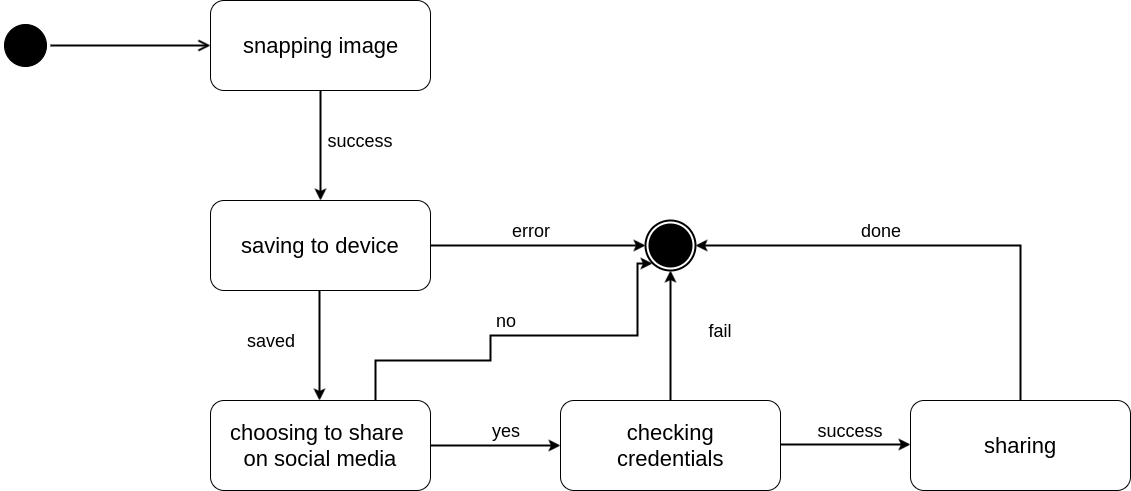
\includegraphics[width=150mm]{SnapshotController.png}
	\caption{SnapshotController}
\end{figure}
\begin{figure}[H]
	\centering
	\includegraphics[width=150mm]{AtmosphericController.png}
	\caption{AtmosphericController}
\end{figure}
\begin{figure}[H]
	\centering
	\includegraphics[width=50mm]{PowerController.png}
	\caption{PowerController}
\end{figure}
\begin{figure}[H]
	\centering
	\includegraphics[width=75mm]{PersonnelController.png}
	\caption{PersonnelController}
\end{figure}
\begin{figure}[H]
	\centering
	\includegraphics[width=150mm]{TopController.png}
	\caption{TopController}
\end{figure}
\begin{figure}[H]
	\centering
	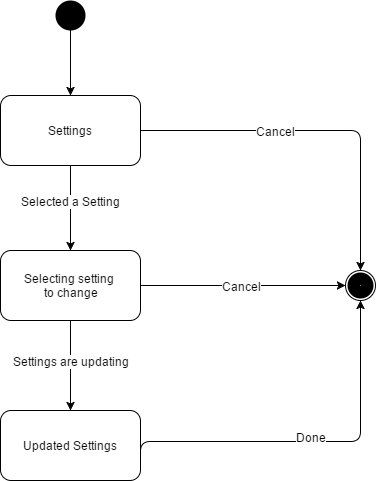
\includegraphics[width=100mm]{SettingsController.png}
	\caption{SettingsController}
\end{figure}


\section{Sequence Diagrams}
\label{sec:sequence_diagrams}
The following is a sequence diagram for each use case scenario of the system.
\begin{figure}[H]
	\centering
	\includegraphics[width=150mm]{UC1-Create-new-station.png}
	\caption{Use Case 1}
\end{figure}
\begin{figure}[H]
	\centering
	\includegraphics[width=150mm]{UC2-Save.png}
	\caption{Use Case 2}
\end{figure}
\begin{figure}[H]
	\centering
	\includegraphics[width=150mm]{UC3-Load.png}
	\caption{Use Case 3}
\end{figure}
\begin{figure}[H]
	\centering
	\includegraphics[width=150mm]{UC4-Change-Setting.png}
	\caption{Use Case 4}
\end{figure}
\begin{figure}[H]
	\centering
	\includegraphics[width=150mm]{UC5-Issue-Order.png}
	\caption{Use Case 5}
\end{figure}
\begin{figure}[H]
	\centering
	\includegraphics[width=150mm]{UC6-Operate-device.png}
	\caption{Use Case 6}
\end{figure}
\begin{figure}[H]
	\centering
	\includegraphics[width=150mm]{UC7-Check-views.png}
	\caption{Use Case 7}
\end{figure}
\begin{figure}[H]
	\centering
	\includegraphics[width=150mm]{UC8-Snapshot.png}
	\caption{Use Case 8}
\end{figure}

\section{Detailed Class Diagram}
\label{sec:detailed_class_diagram}
The following is a detailed class diagram of the system. It has been disconnecting into two pages for readability. The right side of part A's page is intended to connect to the left half of part B's page. Only one configuration that properly connects the two crossing arrows should be possible.
\begin{figure}[H]
	\centering
	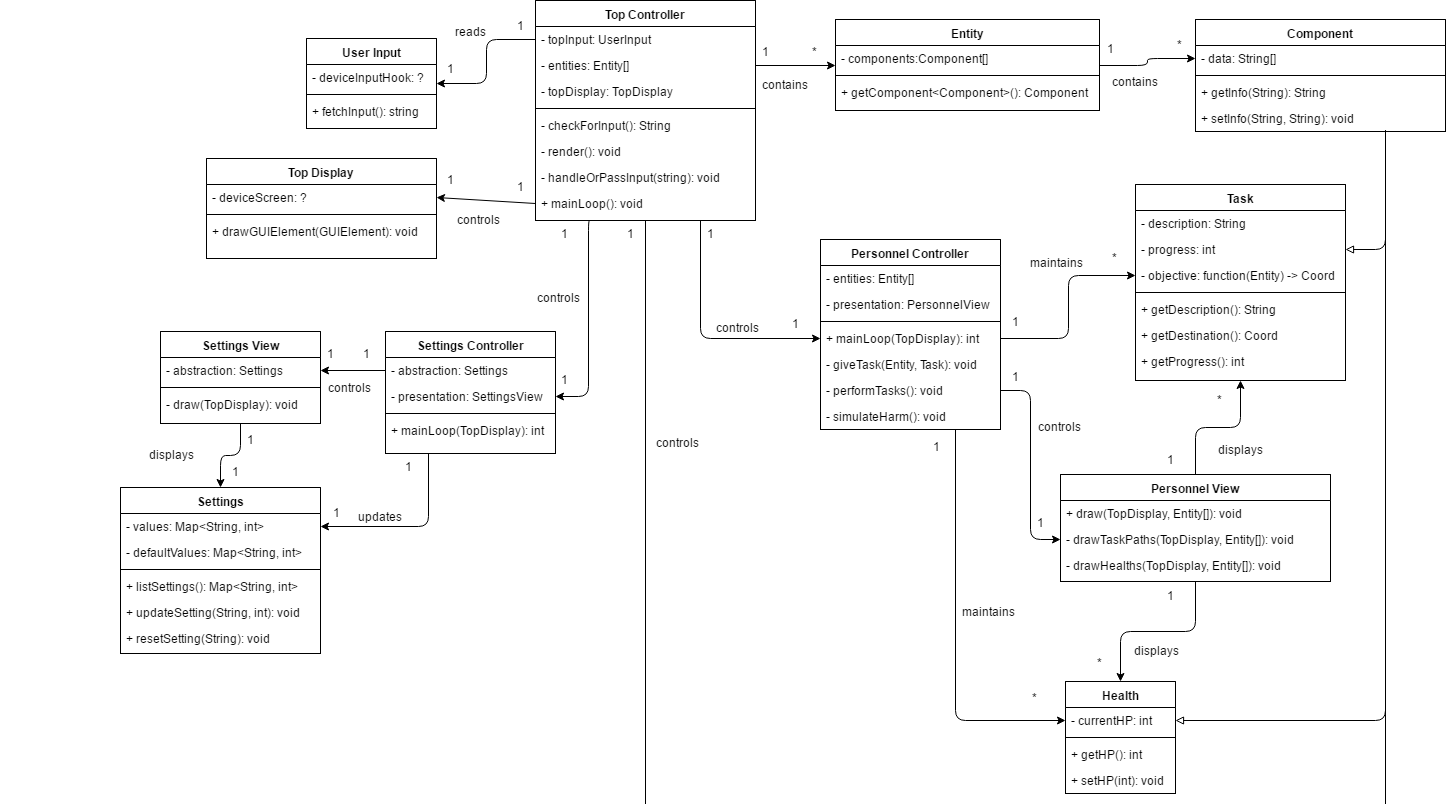
\includegraphics[width=220mm, angle=90]{ClassDiagramA.png}
	\caption{Class Diagram part A}
\end{figure}
\begin{figure}[H]
	\centering
	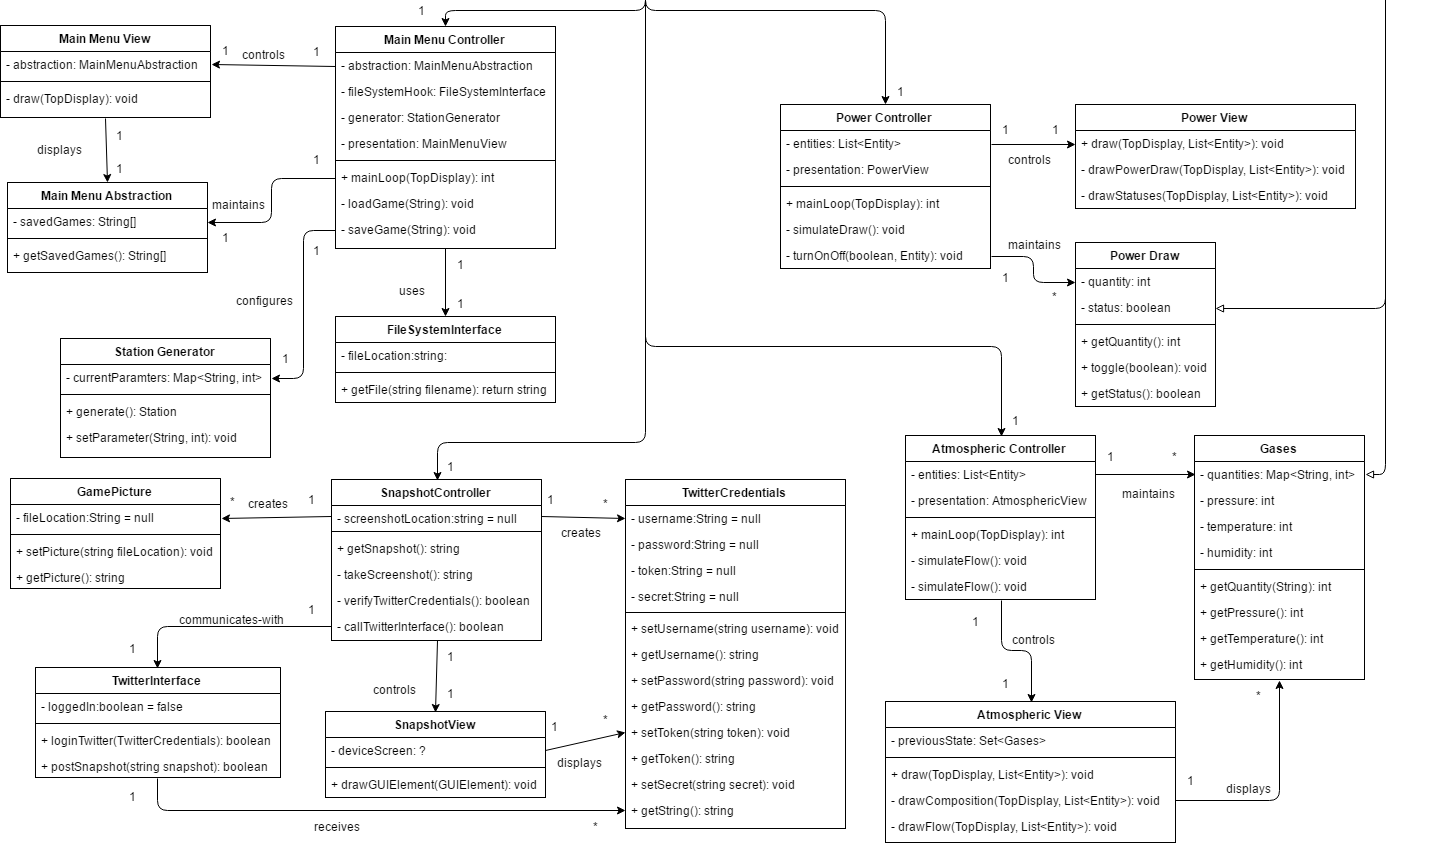
\includegraphics[width=220mm, angle=90]{ClassDiagramB.png}
	\caption{Class Diagram part B}
\end{figure}

\appendix
\section{Division of Labour}
\label{sec:division_of_labour}
The following is a description of the work on this document performed by each team member.
\begin{enumerate}
	\item Ian Prins: Class diagram, introduction, editing
	\item Nishanth Balamohan: State charts
	\item Arfa Amer: Sequence diagrams
	\item Young H. Kim: State charts
	\item Areeb Malik: Class diagram
\end{enumerate}

\end{document}
%------------------------------------------------------------------------------